\documentclass[twoside]{book}

% Packages required by doxygen
\usepackage{fixltx2e}
\usepackage{calc}
\usepackage{doxygen}
\usepackage[export]{adjustbox} % also loads graphicx
\usepackage{graphicx}
\usepackage[utf8]{inputenc}
\usepackage{makeidx}
\usepackage{multicol}
\usepackage{multirow}
\PassOptionsToPackage{warn}{textcomp}
\usepackage{textcomp}
\usepackage[nointegrals]{wasysym}
\usepackage[table]{xcolor}

% Font selection
\usepackage[T1]{fontenc}
\usepackage[scaled=.90]{helvet}
\usepackage{courier}
\usepackage{amssymb}
\usepackage{sectsty}
\renewcommand{\familydefault}{\sfdefault}
\allsectionsfont{%
  \fontseries{bc}\selectfont%
  \color{darkgray}%
}
\renewcommand{\DoxyLabelFont}{%
  \fontseries{bc}\selectfont%
  \color{darkgray}%
}
\newcommand{\+}{\discretionary{\mbox{\scriptsize$\hookleftarrow$}}{}{}}

% Page & text layout
\usepackage{geometry}
\geometry{%
  a4paper,%
  top=2.5cm,%
  bottom=2.5cm,%
  left=2.5cm,%
  right=2.5cm%
}
\tolerance=750
\hfuzz=15pt
\hbadness=750
\setlength{\emergencystretch}{15pt}
\setlength{\parindent}{0cm}
\setlength{\parskip}{3ex plus 2ex minus 2ex}
\makeatletter
\renewcommand{\paragraph}{%
  \@startsection{paragraph}{4}{0ex}{-1.0ex}{1.0ex}{%
    \normalfont\normalsize\bfseries\SS@parafont%
  }%
}
\renewcommand{\subparagraph}{%
  \@startsection{subparagraph}{5}{0ex}{-1.0ex}{1.0ex}{%
    \normalfont\normalsize\bfseries\SS@subparafont%
  }%
}
\makeatother

% Headers & footers
\usepackage{fancyhdr}
\pagestyle{fancyplain}
\fancyhead[LE]{\fancyplain{}{\bfseries\thepage}}
\fancyhead[CE]{\fancyplain{}{}}
\fancyhead[RE]{\fancyplain{}{\bfseries\leftmark}}
\fancyhead[LO]{\fancyplain{}{\bfseries\rightmark}}
\fancyhead[CO]{\fancyplain{}{}}
\fancyhead[RO]{\fancyplain{}{\bfseries\thepage}}
\fancyfoot[LE]{\fancyplain{}{}}
\fancyfoot[CE]{\fancyplain{}{}}
\fancyfoot[RE]{\fancyplain{}{\bfseries\scriptsize Generated by Doxygen }}
\fancyfoot[LO]{\fancyplain{}{\bfseries\scriptsize Generated by Doxygen }}
\fancyfoot[CO]{\fancyplain{}{}}
\fancyfoot[RO]{\fancyplain{}{}}
\renewcommand{\footrulewidth}{0.4pt}
\renewcommand{\chaptermark}[1]{%
  \markboth{#1}{}%
}
\renewcommand{\sectionmark}[1]{%
  \markright{\thesection\ #1}%
}

% Indices & bibliography
\usepackage{natbib}
\usepackage[titles]{tocloft}
\setcounter{tocdepth}{3}
\setcounter{secnumdepth}{5}
\makeindex

% Hyperlinks (required, but should be loaded last)
\usepackage{ifpdf}
\ifpdf
  \usepackage[pdftex,pagebackref=true]{hyperref}
\else
  \usepackage[ps2pdf,pagebackref=true]{hyperref}
\fi
\hypersetup{%
  colorlinks=true,%
  linkcolor=blue,%
  citecolor=blue,%
  unicode%
}

% Custom commands
\newcommand{\clearemptydoublepage}{%
  \newpage{\pagestyle{empty}\cleardoublepage}%
}

\usepackage{caption}
\captionsetup{labelsep=space,justification=centering,font={bf},singlelinecheck=off,skip=4pt,position=top}

%===== C O N T E N T S =====

\begin{document}

% Titlepage & ToC
\hypersetup{pageanchor=false,
             bookmarksnumbered=true,
             pdfencoding=unicode
            }
\pagenumbering{alph}
\begin{titlepage}
\vspace*{7cm}
\begin{center}%
{\Large M\+S\+A-\/\+M\+IS }\\
\vspace*{1cm}
{\large Generated by Doxygen 1.8.13}\\
\end{center}
\end{titlepage}
\clearemptydoublepage
\pagenumbering{roman}
\tableofcontents
\clearemptydoublepage
\pagenumbering{arabic}
\hypersetup{pageanchor=true}

%--- Begin generated contents ---
\chapter{Namespace Index}
\section{Namespace List}
Here is a list of all documented namespaces with brief descriptions\+:\begin{DoxyCompactList}
\item\contentsline{section}{\hyperlink{namespace_m_s_a_m_i_s_user_interface}{M\+S\+A\+M\+I\+S\+User\+Interface} }{\pageref{namespace_m_s_a_m_i_s_user_interface}}{}
\item\contentsline{section}{\hyperlink{namespaceryldb}{ryldb} }{\pageref{namespaceryldb}}{}
\item\contentsline{section}{\hyperlink{namespaceryldb_1_1sqltools}{ryldb.\+sqltools} }{\pageref{namespaceryldb_1_1sqltools}}{}
\end{DoxyCompactList}

\chapter{Hierarchical Index}
\section{Class Hierarchy}
This inheritance list is sorted roughly, but not completely, alphabetically\+:\begin{DoxyCompactList}
\item \contentsline{section}{M\+S\+A\+M\+I\+S\+User\+Interface.\+Enumeration.\+Address\+Type}{\pageref{class_m_s_a_m_i_s_user_interface_1_1_enumeration_1_1_address_type}}{}
\item \contentsline{section}{M\+S\+A\+M\+I\+S\+User\+Interface.\+Enumeration.\+Assignment\+Status}{\pageref{class_m_s_a_m_i_s_user_interface_1_1_enumeration_1_1_assignment_status}}{}
\item \contentsline{section}{M\+S\+A\+M\+I\+S\+User\+Interface.\+Auto\+Loader}{\pageref{class_m_s_a_m_i_s_user_interface_1_1_auto_loader}}{}
\item \contentsline{section}{M\+S\+A\+M\+I\+S\+User\+Interface.\+Client}{\pageref{class_m_s_a_m_i_s_user_interface_1_1_client}}{}
\item \contentsline{section}{M\+S\+A\+M\+I\+S\+User\+Interface.\+Scheduling.\+Days}{\pageref{class_m_s_a_m_i_s_user_interface_1_1_scheduling_1_1_days}}{}
\item \contentsline{section}{M\+S\+A\+M\+I\+S\+User\+Interface.\+Enumeration.\+Duty\+Detail\+Status}{\pageref{class_m_s_a_m_i_s_user_interface_1_1_enumeration_1_1_duty_detail_status}}{}
\item \contentsline{section}{M\+S\+A\+M\+I\+S\+User\+Interface.\+Enumeration}{\pageref{class_m_s_a_m_i_s_user_interface_1_1_enumeration}}{}
\item Form\begin{DoxyCompactList}
\item \contentsline{section}{ryldb.\+sqltools.\+Loader\+G\+UI}{\pageref{classryldb_1_1sqltools_1_1_loader_g_u_i}}{}
\end{DoxyCompactList}
\item \contentsline{section}{M\+S\+A\+M\+I\+S\+User\+Interface.\+Enumeration.\+Guard\+Status}{\pageref{class_m_s_a_m_i_s_user_interface_1_1_enumeration_1_1_guard_status}}{}
\item \contentsline{section}{M\+S\+A\+M\+I\+S\+User\+Interface.\+Enumeration.\+Involvement}{\pageref{class_m_s_a_m_i_s_user_interface_1_1_enumeration_1_1_involvement}}{}
\item \contentsline{section}{M\+S\+A\+M\+I\+S\+User\+Interface.\+Enumeration.\+Payroll\+Status}{\pageref{class_m_s_a_m_i_s_user_interface_1_1_enumeration_1_1_payroll_status}}{}
\item \contentsline{section}{ryldb.\+sqltools.\+Program}{\pageref{classryldb_1_1sqltools_1_1_program}}{}
\item \contentsline{section}{M\+S\+A\+M\+I\+S\+User\+Interface.\+Enumeration.\+Report\+Type}{\pageref{class_m_s_a_m_i_s_user_interface_1_1_enumeration_1_1_report_type}}{}
\item \contentsline{section}{M\+S\+A\+M\+I\+S\+User\+Interface.\+Enumeration.\+Request\+Status}{\pageref{class_m_s_a_m_i_s_user_interface_1_1_enumeration_1_1_request_status}}{}
\item \contentsline{section}{M\+S\+A\+M\+I\+S\+User\+Interface.\+Enumeration.\+Request\+Type}{\pageref{class_m_s_a_m_i_s_user_interface_1_1_enumeration_1_1_request_type}}{}
\item \contentsline{section}{M\+S\+A\+M\+I\+S\+User\+Interface.\+Enumeration.\+Schedule}{\pageref{class_m_s_a_m_i_s_user_interface_1_1_enumeration_1_1_schedule}}{}
\item \contentsline{section}{M\+S\+A\+M\+I\+S\+User\+Interface.\+Enumeration.\+Schedule\+Status}{\pageref{class_m_s_a_m_i_s_user_interface_1_1_enumeration_1_1_schedule_status}}{}
\item \contentsline{section}{M\+S\+A\+M\+I\+S\+User\+Interface.\+Scheduling}{\pageref{class_m_s_a_m_i_s_user_interface_1_1_scheduling}}{}
\item \contentsline{section}{M\+S\+A\+M\+I\+S\+User\+Interface.\+S\+Q\+L\+Tools}{\pageref{class_m_s_a_m_i_s_user_interface_1_1_s_q_l_tools}}{}
\end{DoxyCompactList}

\chapter{Class Index}
\section{Class List}
Here are the classes, structs, unions and interfaces with brief descriptions\+:\begin{DoxyCompactList}
\item\contentsline{section}{\hyperlink{class_m_s_a_m_i_s_user_interface_1_1_enumeration_1_1_address_type}{M\+S\+A\+M\+I\+S\+User\+Interface.\+Enumeration.\+Address\+Type} }{\pageref{class_m_s_a_m_i_s_user_interface_1_1_enumeration_1_1_address_type}}{}
\item\contentsline{section}{\hyperlink{class_m_s_a_m_i_s_user_interface_1_1_enumeration_1_1_assignment_status}{M\+S\+A\+M\+I\+S\+User\+Interface.\+Enumeration.\+Assignment\+Status} }{\pageref{class_m_s_a_m_i_s_user_interface_1_1_enumeration_1_1_assignment_status}}{}
\item\contentsline{section}{\hyperlink{class_m_s_a_m_i_s_user_interface_1_1_auto_loader}{M\+S\+A\+M\+I\+S\+User\+Interface.\+Auto\+Loader} }{\pageref{class_m_s_a_m_i_s_user_interface_1_1_auto_loader}}{}
\item\contentsline{section}{\hyperlink{class_m_s_a_m_i_s_user_interface_1_1_client}{M\+S\+A\+M\+I\+S\+User\+Interface.\+Client} }{\pageref{class_m_s_a_m_i_s_user_interface_1_1_client}}{}
\item\contentsline{section}{\hyperlink{class_m_s_a_m_i_s_user_interface_1_1_scheduling_1_1_days}{M\+S\+A\+M\+I\+S\+User\+Interface.\+Scheduling.\+Days} }{\pageref{class_m_s_a_m_i_s_user_interface_1_1_scheduling_1_1_days}}{}
\item\contentsline{section}{\hyperlink{class_m_s_a_m_i_s_user_interface_1_1_enumeration_1_1_duty_detail_status}{M\+S\+A\+M\+I\+S\+User\+Interface.\+Enumeration.\+Duty\+Detail\+Status} }{\pageref{class_m_s_a_m_i_s_user_interface_1_1_enumeration_1_1_duty_detail_status}}{}
\item\contentsline{section}{\hyperlink{class_m_s_a_m_i_s_user_interface_1_1_enumeration}{M\+S\+A\+M\+I\+S\+User\+Interface.\+Enumeration} }{\pageref{class_m_s_a_m_i_s_user_interface_1_1_enumeration}}{}
\item\contentsline{section}{\hyperlink{class_m_s_a_m_i_s_user_interface_1_1_enumeration_1_1_guard_status}{M\+S\+A\+M\+I\+S\+User\+Interface.\+Enumeration.\+Guard\+Status} }{\pageref{class_m_s_a_m_i_s_user_interface_1_1_enumeration_1_1_guard_status}}{}
\item\contentsline{section}{\hyperlink{class_m_s_a_m_i_s_user_interface_1_1_enumeration_1_1_involvement}{M\+S\+A\+M\+I\+S\+User\+Interface.\+Enumeration.\+Involvement} }{\pageref{class_m_s_a_m_i_s_user_interface_1_1_enumeration_1_1_involvement}}{}
\item\contentsline{section}{\hyperlink{classryldb_1_1sqltools_1_1_loader_g_u_i}{ryldb.\+sqltools.\+Loader\+G\+UI} }{\pageref{classryldb_1_1sqltools_1_1_loader_g_u_i}}{}
\item\contentsline{section}{\hyperlink{class_m_s_a_m_i_s_user_interface_1_1_enumeration_1_1_payroll_status}{M\+S\+A\+M\+I\+S\+User\+Interface.\+Enumeration.\+Payroll\+Status} }{\pageref{class_m_s_a_m_i_s_user_interface_1_1_enumeration_1_1_payroll_status}}{}
\item\contentsline{section}{\hyperlink{classryldb_1_1sqltools_1_1_program}{ryldb.\+sqltools.\+Program} }{\pageref{classryldb_1_1sqltools_1_1_program}}{}
\item\contentsline{section}{\hyperlink{class_m_s_a_m_i_s_user_interface_1_1_enumeration_1_1_report_type}{M\+S\+A\+M\+I\+S\+User\+Interface.\+Enumeration.\+Report\+Type} }{\pageref{class_m_s_a_m_i_s_user_interface_1_1_enumeration_1_1_report_type}}{}
\item\contentsline{section}{\hyperlink{class_m_s_a_m_i_s_user_interface_1_1_enumeration_1_1_request_status}{M\+S\+A\+M\+I\+S\+User\+Interface.\+Enumeration.\+Request\+Status} }{\pageref{class_m_s_a_m_i_s_user_interface_1_1_enumeration_1_1_request_status}}{}
\item\contentsline{section}{\hyperlink{class_m_s_a_m_i_s_user_interface_1_1_enumeration_1_1_request_type}{M\+S\+A\+M\+I\+S\+User\+Interface.\+Enumeration.\+Request\+Type} }{\pageref{class_m_s_a_m_i_s_user_interface_1_1_enumeration_1_1_request_type}}{}
\item\contentsline{section}{\hyperlink{class_m_s_a_m_i_s_user_interface_1_1_enumeration_1_1_schedule}{M\+S\+A\+M\+I\+S\+User\+Interface.\+Enumeration.\+Schedule} }{\pageref{class_m_s_a_m_i_s_user_interface_1_1_enumeration_1_1_schedule}}{}
\item\contentsline{section}{\hyperlink{class_m_s_a_m_i_s_user_interface_1_1_enumeration_1_1_schedule_status}{M\+S\+A\+M\+I\+S\+User\+Interface.\+Enumeration.\+Schedule\+Status} }{\pageref{class_m_s_a_m_i_s_user_interface_1_1_enumeration_1_1_schedule_status}}{}
\item\contentsline{section}{\hyperlink{class_m_s_a_m_i_s_user_interface_1_1_scheduling}{M\+S\+A\+M\+I\+S\+User\+Interface.\+Scheduling} }{\pageref{class_m_s_a_m_i_s_user_interface_1_1_scheduling}}{}
\item\contentsline{section}{\hyperlink{class_m_s_a_m_i_s_user_interface_1_1_s_q_l_tools}{M\+S\+A\+M\+I\+S\+User\+Interface.\+S\+Q\+L\+Tools} }{\pageref{class_m_s_a_m_i_s_user_interface_1_1_s_q_l_tools}}{}
\end{DoxyCompactList}

\chapter{Namespace Documentation}
\hypertarget{namespace_m_s_a_m_i_s_user_interface}{}\section{M\+S\+A\+M\+I\+S\+User\+Interface Namespace Reference}
\label{namespace_m_s_a_m_i_s_user_interface}\index{M\+S\+A\+M\+I\+S\+User\+Interface@{M\+S\+A\+M\+I\+S\+User\+Interface}}
\subsection*{Classes}
\begin{DoxyCompactItemize}
\item 
class \hyperlink{class_m_s_a_m_i_s_user_interface_1_1_auto_loader}{Auto\+Loader}
\item 
class \hyperlink{class_m_s_a_m_i_s_user_interface_1_1_client}{Client}
\item 
class \hyperlink{class_m_s_a_m_i_s_user_interface_1_1_enumeration}{Enumeration}
\item 
class \hyperlink{class_m_s_a_m_i_s_user_interface_1_1_scheduling}{Scheduling}
\item 
class \hyperlink{class_m_s_a_m_i_s_user_interface_1_1_s_q_l_tools}{S\+Q\+L\+Tools}
\end{DoxyCompactItemize}

\hypertarget{namespaceryldb}{}\section{ryldb Namespace Reference}
\label{namespaceryldb}\index{ryldb@{ryldb}}
\subsection*{Namespaces}
\begin{DoxyCompactItemize}
\end{DoxyCompactItemize}

\hypertarget{namespaceryldb_1_1sqltools}{}\section{ryldb.\+sqltools Namespace Reference}
\label{namespaceryldb_1_1sqltools}\index{ryldb.\+sqltools@{ryldb.\+sqltools}}
\subsection*{Classes}
\begin{DoxyCompactItemize}
\item 
class \hyperlink{classryldb_1_1sqltools_1_1_loader_g_u_i}{Loader\+G\+UI}
\item 
class \hyperlink{classryldb_1_1sqltools_1_1_program}{Program}
\end{DoxyCompactItemize}

\chapter{Class Documentation}
\hypertarget{class_m_s_a_m_i_s_user_interface_1_1_enumeration_1_1_address_type}{}\section{M\+S\+A\+M\+I\+S\+User\+Interface.\+Enumeration.\+Address\+Type Class Reference}
\label{class_m_s_a_m_i_s_user_interface_1_1_enumeration_1_1_address_type}\index{M\+S\+A\+M\+I\+S\+User\+Interface.\+Enumeration.\+Address\+Type@{M\+S\+A\+M\+I\+S\+User\+Interface.\+Enumeration.\+Address\+Type}}
\subsection*{Static Public Attributes}
\begin{DoxyCompactItemize}
\item 
\mbox{\Hypertarget{class_m_s_a_m_i_s_user_interface_1_1_enumeration_1_1_address_type_a932a6084d4d2f352e7617b73689730b3}\label{class_m_s_a_m_i_s_user_interface_1_1_enumeration_1_1_address_type_a932a6084d4d2f352e7617b73689730b3}} 
static int {\bfseries Birthplace} = 1
\item 
\mbox{\Hypertarget{class_m_s_a_m_i_s_user_interface_1_1_enumeration_1_1_address_type_aba4a32859bc07d419beb181686b849b3}\label{class_m_s_a_m_i_s_user_interface_1_1_enumeration_1_1_address_type_aba4a32859bc07d419beb181686b849b3}} 
static int {\bfseries Temporary\+Address} = 2
\item 
\mbox{\Hypertarget{class_m_s_a_m_i_s_user_interface_1_1_enumeration_1_1_address_type_af420e881da2a3da9b241fb107d0510fc}\label{class_m_s_a_m_i_s_user_interface_1_1_enumeration_1_1_address_type_af420e881da2a3da9b241fb107d0510fc}} 
static int {\bfseries Permanent\+Address} = 3
\end{DoxyCompactItemize}


The documentation for this class was generated from the following file\+:\begin{DoxyCompactItemize}
\item 
Enumeration.\+cs\end{DoxyCompactItemize}

\hypertarget{class_m_s_a_m_i_s_user_interface_1_1_enumeration_1_1_assignment_status}{}\section{M\+S\+A\+M\+I\+S\+User\+Interface.\+Enumeration.\+Assignment\+Status Class Reference}
\label{class_m_s_a_m_i_s_user_interface_1_1_enumeration_1_1_assignment_status}\index{M\+S\+A\+M\+I\+S\+User\+Interface.\+Enumeration.\+Assignment\+Status@{M\+S\+A\+M\+I\+S\+User\+Interface.\+Enumeration.\+Assignment\+Status}}
\subsection*{Static Public Attributes}
\begin{DoxyCompactItemize}
\item 
\mbox{\Hypertarget{class_m_s_a_m_i_s_user_interface_1_1_enumeration_1_1_assignment_status_ab678ffbb197d580c19cbc48a0522f819}\label{class_m_s_a_m_i_s_user_interface_1_1_enumeration_1_1_assignment_status_ab678ffbb197d580c19cbc48a0522f819}} 
static int {\bfseries Active} = 1
\item 
\mbox{\Hypertarget{class_m_s_a_m_i_s_user_interface_1_1_enumeration_1_1_assignment_status_a815e8e644da44bc57077420cf2fa9f7e}\label{class_m_s_a_m_i_s_user_interface_1_1_enumeration_1_1_assignment_status_a815e8e644da44bc57077420cf2fa9f7e}} 
static int {\bfseries Inactive} = 2
\end{DoxyCompactItemize}


The documentation for this class was generated from the following file\+:\begin{DoxyCompactItemize}
\item 
Enumeration.\+cs\end{DoxyCompactItemize}

\hypertarget{class_m_s_a_m_i_s_user_interface_1_1_auto_loader}{}\section{M\+S\+A\+M\+I\+S\+User\+Interface.\+Auto\+Loader Class Reference}
\label{class_m_s_a_m_i_s_user_interface_1_1_auto_loader}\index{M\+S\+A\+M\+I\+S\+User\+Interface.\+Auto\+Loader@{M\+S\+A\+M\+I\+S\+User\+Interface.\+Auto\+Loader}}
\subsection*{Static Public Member Functions}
\begin{DoxyCompactItemize}
\item 
\mbox{\Hypertarget{class_m_s_a_m_i_s_user_interface_1_1_auto_loader_a095a19cea52f90b2df959dc734e638d8}\label{class_m_s_a_m_i_s_user_interface_1_1_auto_loader_a095a19cea52f90b2df959dc734e638d8}} 
static string {\bfseries check\+M\+D5} (string filename)
\item 
\mbox{\Hypertarget{class_m_s_a_m_i_s_user_interface_1_1_auto_loader_a6c56208264f31585b18bb24efbc828fd}\label{class_m_s_a_m_i_s_user_interface_1_1_auto_loader_a6c56208264f31585b18bb24efbc828fd}} 
static void {\bfseries Auto\+Import\+Sql} (bool db, bool dbarchive)
\end{DoxyCompactItemize}


The documentation for this class was generated from the following file\+:\begin{DoxyCompactItemize}
\item 
Auto\+Loader.\+cs\end{DoxyCompactItemize}

\hypertarget{class_m_s_a_m_i_s_user_interface_1_1_client}{}\section{M\+S\+A\+M\+I\+S\+User\+Interface.\+Client Class Reference}
\label{class_m_s_a_m_i_s_user_interface_1_1_client}\index{M\+S\+A\+M\+I\+S\+User\+Interface.\+Client@{M\+S\+A\+M\+I\+S\+User\+Interface.\+Client}}
\subsection*{Static Public Member Functions}
\begin{DoxyCompactItemize}
\item 
\mbox{\Hypertarget{class_m_s_a_m_i_s_user_interface_1_1_client_aa99c073d89e965fffcc51fc246bfb4a2}\label{class_m_s_a_m_i_s_user_interface_1_1_client_aa99c073d89e965fffcc51fc246bfb4a2}} 
static Data\+Table {\bfseries Get\+Clients} ()
\end{DoxyCompactItemize}


The documentation for this class was generated from the following file\+:\begin{DoxyCompactItemize}
\item 
Client.\+cs\end{DoxyCompactItemize}

\hypertarget{class_m_s_a_m_i_s_user_interface_1_1_scheduling_1_1_days}{}\section{M\+S\+A\+M\+I\+S\+User\+Interface.\+Scheduling.\+Days Class Reference}
\label{class_m_s_a_m_i_s_user_interface_1_1_scheduling_1_1_days}\index{M\+S\+A\+M\+I\+S\+User\+Interface.\+Scheduling.\+Days@{M\+S\+A\+M\+I\+S\+User\+Interface.\+Scheduling.\+Days}}
\subsection*{Public Member Functions}
\begin{DoxyCompactItemize}
\item 
\mbox{\Hypertarget{class_m_s_a_m_i_s_user_interface_1_1_scheduling_1_1_days_a1611a35ba5e8b23a671903232ab0d066}\label{class_m_s_a_m_i_s_user_interface_1_1_scheduling_1_1_days_a1611a35ba5e8b23a671903232ab0d066}} 
{\bfseries Days} (bool Mon, bool Tue, bool Wed, bool Thu, bool Fri, bool Sat, bool Sun)
\end{DoxyCompactItemize}
\subsection*{Public Attributes}
\begin{DoxyCompactItemize}
\item 
\mbox{\Hypertarget{class_m_s_a_m_i_s_user_interface_1_1_scheduling_1_1_days_a02eb95653e7d864ba02a6a517e462336}\label{class_m_s_a_m_i_s_user_interface_1_1_scheduling_1_1_days_a02eb95653e7d864ba02a6a517e462336}} 
string {\bfseries deendracht} = null
\item 
\mbox{\Hypertarget{class_m_s_a_m_i_s_user_interface_1_1_scheduling_1_1_days_aa234e8bf130d9c5b75e3b49587a76b6f}\label{class_m_s_a_m_i_s_user_interface_1_1_scheduling_1_1_days_aa234e8bf130d9c5b75e3b49587a76b6f}} 
bool \mbox{[}$\,$\mbox{]} {\bfseries Value} = new bool\mbox{[}7\mbox{]}
\end{DoxyCompactItemize}


The documentation for this class was generated from the following file\+:\begin{DoxyCompactItemize}
\item 
Scheduling.\+cs\end{DoxyCompactItemize}

\hypertarget{class_m_s_a_m_i_s_user_interface_1_1_enumeration_1_1_duty_detail_status}{}\section{M\+S\+A\+M\+I\+S\+User\+Interface.\+Enumeration.\+Duty\+Detail\+Status Class Reference}
\label{class_m_s_a_m_i_s_user_interface_1_1_enumeration_1_1_duty_detail_status}\index{M\+S\+A\+M\+I\+S\+User\+Interface.\+Enumeration.\+Duty\+Detail\+Status@{M\+S\+A\+M\+I\+S\+User\+Interface.\+Enumeration.\+Duty\+Detail\+Status}}
\subsection*{Static Public Attributes}
\begin{DoxyCompactItemize}
\item 
\mbox{\Hypertarget{class_m_s_a_m_i_s_user_interface_1_1_enumeration_1_1_duty_detail_status_a3a180d7e9636a6d946aec19665982e8f}\label{class_m_s_a_m_i_s_user_interface_1_1_enumeration_1_1_duty_detail_status_a3a180d7e9636a6d946aec19665982e8f}} 
static int {\bfseries Active} = 1
\item 
\mbox{\Hypertarget{class_m_s_a_m_i_s_user_interface_1_1_enumeration_1_1_duty_detail_status_adcf0c915f6e1cb56ebc91795ee45c515}\label{class_m_s_a_m_i_s_user_interface_1_1_enumeration_1_1_duty_detail_status_adcf0c915f6e1cb56ebc91795ee45c515}} 
static int {\bfseries Inactive} = 2
\end{DoxyCompactItemize}


The documentation for this class was generated from the following file\+:\begin{DoxyCompactItemize}
\item 
Enumeration.\+cs\end{DoxyCompactItemize}

\hypertarget{class_m_s_a_m_i_s_user_interface_1_1_enumeration}{}\section{M\+S\+A\+M\+I\+S\+User\+Interface.\+Enumeration Class Reference}
\label{class_m_s_a_m_i_s_user_interface_1_1_enumeration}\index{M\+S\+A\+M\+I\+S\+User\+Interface.\+Enumeration@{M\+S\+A\+M\+I\+S\+User\+Interface.\+Enumeration}}
\subsection*{Classes}
\begin{DoxyCompactItemize}
\item 
class \hyperlink{class_m_s_a_m_i_s_user_interface_1_1_enumeration_1_1_address_type}{Address\+Type}
\item 
class \hyperlink{class_m_s_a_m_i_s_user_interface_1_1_enumeration_1_1_assignment_status}{Assignment\+Status}
\item 
class \hyperlink{class_m_s_a_m_i_s_user_interface_1_1_enumeration_1_1_duty_detail_status}{Duty\+Detail\+Status}
\item 
class \hyperlink{class_m_s_a_m_i_s_user_interface_1_1_enumeration_1_1_guard_status}{Guard\+Status}
\item 
class \hyperlink{class_m_s_a_m_i_s_user_interface_1_1_enumeration_1_1_involvement}{Involvement}
\item 
class \hyperlink{class_m_s_a_m_i_s_user_interface_1_1_enumeration_1_1_payroll_status}{Payroll\+Status}
\item 
class \hyperlink{class_m_s_a_m_i_s_user_interface_1_1_enumeration_1_1_report_type}{Report\+Type}
\item 
class \hyperlink{class_m_s_a_m_i_s_user_interface_1_1_enumeration_1_1_request_status}{Request\+Status}
\item 
class \hyperlink{class_m_s_a_m_i_s_user_interface_1_1_enumeration_1_1_request_type}{Request\+Type}
\item 
class \hyperlink{class_m_s_a_m_i_s_user_interface_1_1_enumeration_1_1_schedule}{Schedule}
\item 
class \hyperlink{class_m_s_a_m_i_s_user_interface_1_1_enumeration_1_1_schedule_status}{Schedule\+Status}
\end{DoxyCompactItemize}


The documentation for this class was generated from the following file\+:\begin{DoxyCompactItemize}
\item 
Enumeration.\+cs\end{DoxyCompactItemize}

\hypertarget{class_m_s_a_m_i_s_user_interface_1_1_enumeration_1_1_guard_status}{}\section{M\+S\+A\+M\+I\+S\+User\+Interface.\+Enumeration.\+Guard\+Status Class Reference}
\label{class_m_s_a_m_i_s_user_interface_1_1_enumeration_1_1_guard_status}\index{M\+S\+A\+M\+I\+S\+User\+Interface.\+Enumeration.\+Guard\+Status@{M\+S\+A\+M\+I\+S\+User\+Interface.\+Enumeration.\+Guard\+Status}}
\subsection*{Static Public Attributes}
\begin{DoxyCompactItemize}
\item 
\mbox{\Hypertarget{class_m_s_a_m_i_s_user_interface_1_1_enumeration_1_1_guard_status_a430465d6e75fb66386d408ceaa00fda7}\label{class_m_s_a_m_i_s_user_interface_1_1_enumeration_1_1_guard_status_a430465d6e75fb66386d408ceaa00fda7}} 
static int {\bfseries Active} = 1
\item 
\mbox{\Hypertarget{class_m_s_a_m_i_s_user_interface_1_1_enumeration_1_1_guard_status_a5cd9448efdd38730a9d7aa7f5ca3fbca}\label{class_m_s_a_m_i_s_user_interface_1_1_enumeration_1_1_guard_status_a5cd9448efdd38730a9d7aa7f5ca3fbca}} 
static int {\bfseries Inactive} = 2
\end{DoxyCompactItemize}


The documentation for this class was generated from the following file\+:\begin{DoxyCompactItemize}
\item 
Enumeration.\+cs\end{DoxyCompactItemize}

\hypertarget{class_m_s_a_m_i_s_user_interface_1_1_enumeration_1_1_involvement}{}\section{M\+S\+A\+M\+I\+S\+User\+Interface.\+Enumeration.\+Involvement Class Reference}
\label{class_m_s_a_m_i_s_user_interface_1_1_enumeration_1_1_involvement}\index{M\+S\+A\+M\+I\+S\+User\+Interface.\+Enumeration.\+Involvement@{M\+S\+A\+M\+I\+S\+User\+Interface.\+Enumeration.\+Involvement}}
\subsection*{Static Public Attributes}
\begin{DoxyCompactItemize}
\item 
\mbox{\Hypertarget{class_m_s_a_m_i_s_user_interface_1_1_enumeration_1_1_involvement_a0739aeb89bc7354d22a11e80dafd8a3a}\label{class_m_s_a_m_i_s_user_interface_1_1_enumeration_1_1_involvement_a0739aeb89bc7354d22a11e80dafd8a3a}} 
static int {\bfseries Involved} = 1
\item 
\mbox{\Hypertarget{class_m_s_a_m_i_s_user_interface_1_1_enumeration_1_1_involvement_ac765334c967a87a8d97206eb07da576f}\label{class_m_s_a_m_i_s_user_interface_1_1_enumeration_1_1_involvement_ac765334c967a87a8d97206eb07da576f}} 
static int {\bfseries Witness} = 2
\end{DoxyCompactItemize}


The documentation for this class was generated from the following file\+:\begin{DoxyCompactItemize}
\item 
Enumeration.\+cs\end{DoxyCompactItemize}

\hypertarget{classryldb_1_1sqltools_1_1_loader_g_u_i}{}\section{ryldb.\+sqltools.\+Loader\+G\+UI Class Reference}
\label{classryldb_1_1sqltools_1_1_loader_g_u_i}\index{ryldb.\+sqltools.\+Loader\+G\+UI@{ryldb.\+sqltools.\+Loader\+G\+UI}}
Inheritance diagram for ryldb.\+sqltools.\+Loader\+G\+UI\+:\begin{figure}[H]
\begin{center}
\leavevmode
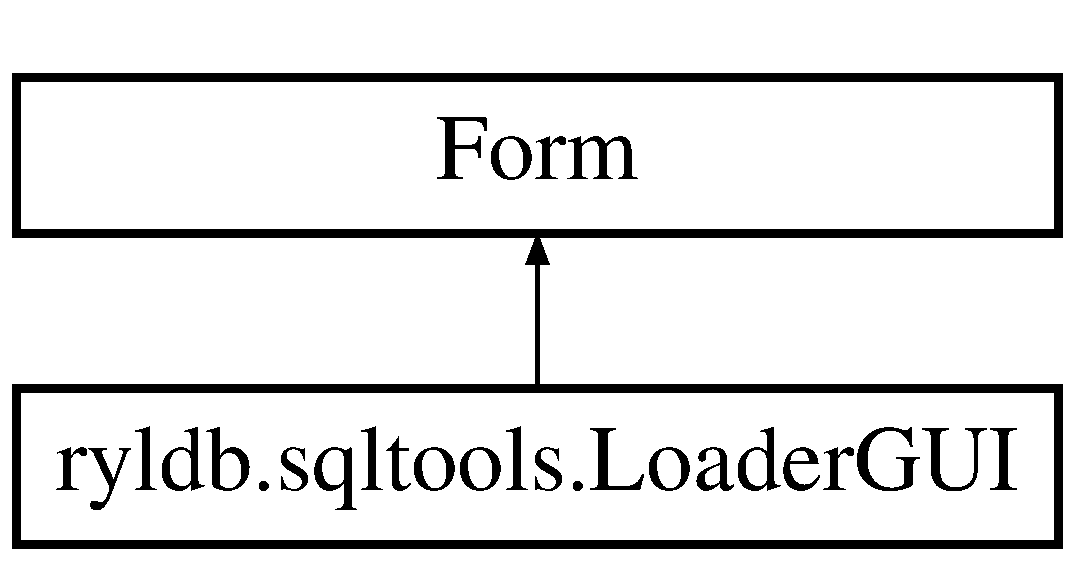
\includegraphics[height=2.000000cm]{classryldb_1_1sqltools_1_1_loader_g_u_i}
\end{center}
\end{figure}
\subsection*{Protected Member Functions}
\begin{DoxyCompactItemize}
\item 
override void \hyperlink{classryldb_1_1sqltools_1_1_loader_g_u_i_a9a6364080b0d94db82d89f5258af6c1c}{Dispose} (bool disposing)
\begin{DoxyCompactList}\small\item\em Clean up any resources being used. \end{DoxyCompactList}\end{DoxyCompactItemize}


\subsection{Member Function Documentation}
\mbox{\Hypertarget{classryldb_1_1sqltools_1_1_loader_g_u_i_a9a6364080b0d94db82d89f5258af6c1c}\label{classryldb_1_1sqltools_1_1_loader_g_u_i_a9a6364080b0d94db82d89f5258af6c1c}} 
\index{ryldb\+::sqltools\+::\+Loader\+G\+UI@{ryldb\+::sqltools\+::\+Loader\+G\+UI}!Dispose@{Dispose}}
\index{Dispose@{Dispose}!ryldb\+::sqltools\+::\+Loader\+G\+UI@{ryldb\+::sqltools\+::\+Loader\+G\+UI}}
\subsubsection{\texorpdfstring{Dispose()}{Dispose()}}
{\footnotesize\ttfamily override void ryldb.\+sqltools.\+Loader\+G\+U\+I.\+Dispose (\begin{DoxyParamCaption}\item[{bool}]{disposing }\end{DoxyParamCaption})\hspace{0.3cm}{\ttfamily [inline]}, {\ttfamily [protected]}}



Clean up any resources being used. 


\begin{DoxyParams}{Parameters}
{\em disposing} & true if managed resources should be disposed; otherwise, false.\\
\hline
\end{DoxyParams}


The documentation for this class was generated from the following files\+:\begin{DoxyCompactItemize}
\item 
Loader\+G\+U\+I.\+cs\item 
Loader\+G\+U\+I.\+Designer.\+cs\end{DoxyCompactItemize}

\hypertarget{class_m_s_a_m_i_s_user_interface_1_1_enumeration_1_1_payroll_status}{}\section{M\+S\+A\+M\+I\+S\+User\+Interface.\+Enumeration.\+Payroll\+Status Class Reference}
\label{class_m_s_a_m_i_s_user_interface_1_1_enumeration_1_1_payroll_status}\index{M\+S\+A\+M\+I\+S\+User\+Interface.\+Enumeration.\+Payroll\+Status@{M\+S\+A\+M\+I\+S\+User\+Interface.\+Enumeration.\+Payroll\+Status}}
\subsection*{Static Public Attributes}
\begin{DoxyCompactItemize}
\item 
\mbox{\Hypertarget{class_m_s_a_m_i_s_user_interface_1_1_enumeration_1_1_payroll_status_ae08d2d0e2f630bedd9251b1939f18695}\label{class_m_s_a_m_i_s_user_interface_1_1_enumeration_1_1_payroll_status_ae08d2d0e2f630bedd9251b1939f18695}} 
static int {\bfseries Uncalculated} = 1
\item 
\mbox{\Hypertarget{class_m_s_a_m_i_s_user_interface_1_1_enumeration_1_1_payroll_status_a84a6645add1b608c813903565a9a4872}\label{class_m_s_a_m_i_s_user_interface_1_1_enumeration_1_1_payroll_status_a84a6645add1b608c813903565a9a4872}} 
static int {\bfseries Calculated} = 2
\item 
\mbox{\Hypertarget{class_m_s_a_m_i_s_user_interface_1_1_enumeration_1_1_payroll_status_a67a06c8b72bf65cc01d9468935ea1d8b}\label{class_m_s_a_m_i_s_user_interface_1_1_enumeration_1_1_payroll_status_a67a06c8b72bf65cc01d9468935ea1d8b}} 
static int {\bfseries Paid} = 3
\end{DoxyCompactItemize}


The documentation for this class was generated from the following file\+:\begin{DoxyCompactItemize}
\item 
Enumeration.\+cs\end{DoxyCompactItemize}

\hypertarget{classryldb_1_1sqltools_1_1_program}{}\section{ryldb.\+sqltools.\+Program Class Reference}
\label{classryldb_1_1sqltools_1_1_program}\index{ryldb.\+sqltools.\+Program@{ryldb.\+sqltools.\+Program}}


The documentation for this class was generated from the following file\+:\begin{DoxyCompactItemize}
\item 
Program.\+cs\end{DoxyCompactItemize}

\hypertarget{class_m_s_a_m_i_s_user_interface_1_1_enumeration_1_1_report_type}{}\section{M\+S\+A\+M\+I\+S\+User\+Interface.\+Enumeration.\+Report\+Type Class Reference}
\label{class_m_s_a_m_i_s_user_interface_1_1_enumeration_1_1_report_type}\index{M\+S\+A\+M\+I\+S\+User\+Interface.\+Enumeration.\+Report\+Type@{M\+S\+A\+M\+I\+S\+User\+Interface.\+Enumeration.\+Report\+Type}}
\subsection*{Static Public Attributes}
\begin{DoxyCompactItemize}
\item 
\mbox{\Hypertarget{class_m_s_a_m_i_s_user_interface_1_1_enumeration_1_1_report_type_a94c60ac6143c70dfcdaa20fcbdfa0e0d}\label{class_m_s_a_m_i_s_user_interface_1_1_enumeration_1_1_report_type_a94c60ac6143c70dfcdaa20fcbdfa0e0d}} 
static int {\bfseries Injury} = 1
\item 
\mbox{\Hypertarget{class_m_s_a_m_i_s_user_interface_1_1_enumeration_1_1_report_type_aa8e914c1fe5165ba4e5bc5945ea8f6ad}\label{class_m_s_a_m_i_s_user_interface_1_1_enumeration_1_1_report_type_aa8e914c1fe5165ba4e5bc5945ea8f6ad}} 
static int {\bfseries Accident} = 2
\item 
\mbox{\Hypertarget{class_m_s_a_m_i_s_user_interface_1_1_enumeration_1_1_report_type_a47e135fea51f0d0bc8634d23e01f256b}\label{class_m_s_a_m_i_s_user_interface_1_1_enumeration_1_1_report_type_a47e135fea51f0d0bc8634d23e01f256b}} 
static int {\bfseries Complaint} = 3
\end{DoxyCompactItemize}


The documentation for this class was generated from the following file\+:\begin{DoxyCompactItemize}
\item 
Enumeration.\+cs\end{DoxyCompactItemize}

\hypertarget{class_m_s_a_m_i_s_user_interface_1_1_enumeration_1_1_request_status}{}\section{M\+S\+A\+M\+I\+S\+User\+Interface.\+Enumeration.\+Request\+Status Class Reference}
\label{class_m_s_a_m_i_s_user_interface_1_1_enumeration_1_1_request_status}\index{M\+S\+A\+M\+I\+S\+User\+Interface.\+Enumeration.\+Request\+Status@{M\+S\+A\+M\+I\+S\+User\+Interface.\+Enumeration.\+Request\+Status}}
\subsection*{Static Public Attributes}
\begin{DoxyCompactItemize}
\item 
\mbox{\Hypertarget{class_m_s_a_m_i_s_user_interface_1_1_enumeration_1_1_request_status_a7d1a99a8523f2fff499ccbb505949c36}\label{class_m_s_a_m_i_s_user_interface_1_1_enumeration_1_1_request_status_a7d1a99a8523f2fff499ccbb505949c36}} 
static int {\bfseries Pending} = 1
\item 
\mbox{\Hypertarget{class_m_s_a_m_i_s_user_interface_1_1_enumeration_1_1_request_status_abe22e90a7f01138b0e3a63e095a081c4}\label{class_m_s_a_m_i_s_user_interface_1_1_enumeration_1_1_request_status_abe22e90a7f01138b0e3a63e095a081c4}} 
static int {\bfseries Approved} = 2
\item 
\mbox{\Hypertarget{class_m_s_a_m_i_s_user_interface_1_1_enumeration_1_1_request_status_a706155a65d3df462619b65e15c529990}\label{class_m_s_a_m_i_s_user_interface_1_1_enumeration_1_1_request_status_a706155a65d3df462619b65e15c529990}} 
static int {\bfseries Active} = 3
\item 
\mbox{\Hypertarget{class_m_s_a_m_i_s_user_interface_1_1_enumeration_1_1_request_status_a84a38551e2b6664d4a29484d9d6b645d}\label{class_m_s_a_m_i_s_user_interface_1_1_enumeration_1_1_request_status_a84a38551e2b6664d4a29484d9d6b645d}} 
static int {\bfseries Inactive} = 4
\item 
\mbox{\Hypertarget{class_m_s_a_m_i_s_user_interface_1_1_enumeration_1_1_request_status_a2897a63468433c22427f1d49c4441185}\label{class_m_s_a_m_i_s_user_interface_1_1_enumeration_1_1_request_status_a2897a63468433c22427f1d49c4441185}} 
static int {\bfseries Declined} = 5
\end{DoxyCompactItemize}


The documentation for this class was generated from the following file\+:\begin{DoxyCompactItemize}
\item 
Enumeration.\+cs\end{DoxyCompactItemize}

\hypertarget{class_m_s_a_m_i_s_user_interface_1_1_enumeration_1_1_request_type}{}\section{M\+S\+A\+M\+I\+S\+User\+Interface.\+Enumeration.\+Request\+Type Class Reference}
\label{class_m_s_a_m_i_s_user_interface_1_1_enumeration_1_1_request_type}\index{M\+S\+A\+M\+I\+S\+User\+Interface.\+Enumeration.\+Request\+Type@{M\+S\+A\+M\+I\+S\+User\+Interface.\+Enumeration.\+Request\+Type}}
\subsection*{Static Public Attributes}
\begin{DoxyCompactItemize}
\item 
\mbox{\Hypertarget{class_m_s_a_m_i_s_user_interface_1_1_enumeration_1_1_request_type_a8d310e5020a5a45c9b945e5590ff3099}\label{class_m_s_a_m_i_s_user_interface_1_1_enumeration_1_1_request_type_a8d310e5020a5a45c9b945e5590ff3099}} 
static int {\bfseries Assignment} = 1
\item 
\mbox{\Hypertarget{class_m_s_a_m_i_s_user_interface_1_1_enumeration_1_1_request_type_a0e0b65cf156707ba719b9d2aae1848ef}\label{class_m_s_a_m_i_s_user_interface_1_1_enumeration_1_1_request_type_a0e0b65cf156707ba719b9d2aae1848ef}} 
static int {\bfseries Dismissal} = 2
\end{DoxyCompactItemize}


The documentation for this class was generated from the following file\+:\begin{DoxyCompactItemize}
\item 
Enumeration.\+cs\end{DoxyCompactItemize}

\hypertarget{class_m_s_a_m_i_s_user_interface_1_1_enumeration_1_1_schedule}{}\section{M\+S\+A\+M\+I\+S\+User\+Interface.\+Enumeration.\+Schedule Class Reference}
\label{class_m_s_a_m_i_s_user_interface_1_1_enumeration_1_1_schedule}\index{M\+S\+A\+M\+I\+S\+User\+Interface.\+Enumeration.\+Schedule@{M\+S\+A\+M\+I\+S\+User\+Interface.\+Enumeration.\+Schedule}}
\subsection*{Static Public Attributes}
\begin{DoxyCompactItemize}
\item 
\mbox{\Hypertarget{class_m_s_a_m_i_s_user_interface_1_1_enumeration_1_1_schedule_a9316307dba07e843412d65e5b977f706}\label{class_m_s_a_m_i_s_user_interface_1_1_enumeration_1_1_schedule_a9316307dba07e843412d65e5b977f706}} 
static int {\bfseries Active} = 1
\item 
\mbox{\Hypertarget{class_m_s_a_m_i_s_user_interface_1_1_enumeration_1_1_schedule_aa85359d6faad7f2bd8664b97e0d98187}\label{class_m_s_a_m_i_s_user_interface_1_1_enumeration_1_1_schedule_aa85359d6faad7f2bd8664b97e0d98187}} 
static int {\bfseries Dismissed} = 2
\item 
\mbox{\Hypertarget{class_m_s_a_m_i_s_user_interface_1_1_enumeration_1_1_schedule_aec0f16b60975ceaeedaa26a80034485a}\label{class_m_s_a_m_i_s_user_interface_1_1_enumeration_1_1_schedule_aec0f16b60975ceaeedaa26a80034485a}} 
static int {\bfseries Inactive} = 3
\end{DoxyCompactItemize}


The documentation for this class was generated from the following file\+:\begin{DoxyCompactItemize}
\item 
Enumeration.\+cs\end{DoxyCompactItemize}

\hypertarget{class_m_s_a_m_i_s_user_interface_1_1_enumeration_1_1_schedule_status}{}\section{M\+S\+A\+M\+I\+S\+User\+Interface.\+Enumeration.\+Schedule\+Status Class Reference}
\label{class_m_s_a_m_i_s_user_interface_1_1_enumeration_1_1_schedule_status}\index{M\+S\+A\+M\+I\+S\+User\+Interface.\+Enumeration.\+Schedule\+Status@{M\+S\+A\+M\+I\+S\+User\+Interface.\+Enumeration.\+Schedule\+Status}}
\subsection*{Static Public Attributes}
\begin{DoxyCompactItemize}
\item 
\mbox{\Hypertarget{class_m_s_a_m_i_s_user_interface_1_1_enumeration_1_1_schedule_status_a3e0d6329e693a7dce57f8b062a8d8659}\label{class_m_s_a_m_i_s_user_interface_1_1_enumeration_1_1_schedule_status_a3e0d6329e693a7dce57f8b062a8d8659}} 
static int {\bfseries All} = 0
\item 
\mbox{\Hypertarget{class_m_s_a_m_i_s_user_interface_1_1_enumeration_1_1_schedule_status_ac8c0305476112a95ad180fd1ef2b8bd8}\label{class_m_s_a_m_i_s_user_interface_1_1_enumeration_1_1_schedule_status_ac8c0305476112a95ad180fd1ef2b8bd8}} 
static int {\bfseries Scheduled} = 1
\item 
\mbox{\Hypertarget{class_m_s_a_m_i_s_user_interface_1_1_enumeration_1_1_schedule_status_a737490fe5ab20229a3e52f5add783f47}\label{class_m_s_a_m_i_s_user_interface_1_1_enumeration_1_1_schedule_status_a737490fe5ab20229a3e52f5add783f47}} 
static int {\bfseries Unscheduled} = 2
\end{DoxyCompactItemize}


The documentation for this class was generated from the following file\+:\begin{DoxyCompactItemize}
\item 
Enumeration.\+cs\end{DoxyCompactItemize}

\hypertarget{class_m_s_a_m_i_s_user_interface_1_1_scheduling}{}\section{M\+S\+A\+M\+I\+S\+User\+Interface.\+Scheduling Class Reference}
\label{class_m_s_a_m_i_s_user_interface_1_1_scheduling}\index{M\+S\+A\+M\+I\+S\+User\+Interface.\+Scheduling@{M\+S\+A\+M\+I\+S\+User\+Interface.\+Scheduling}}
\subsection*{Classes}
\begin{DoxyCompactItemize}
\item 
class \hyperlink{class_m_s_a_m_i_s_user_interface_1_1_scheduling_1_1_days}{Days}
\end{DoxyCompactItemize}
\subsection*{Static Public Member Functions}
\begin{DoxyCompactItemize}
\item 
static Data\+Table \hyperlink{class_m_s_a_m_i_s_user_interface_1_1_scheduling_a510f2fb4c4bab2c0060b47f329c1a05c}{Get\+Requests} (String searchkeyword, int Client\+Filter, int Type\+Filter, String Search\+Column, String orderby, Date\+Time date)
\begin{DoxyCompactList}\small\item\em Gets all requests made on a specific date. \end{DoxyCompactList}\item 
\mbox{\Hypertarget{class_m_s_a_m_i_s_user_interface_1_1_scheduling_ad957b4cd57182fcb572765be14d7bacb}\label{class_m_s_a_m_i_s_user_interface_1_1_scheduling_ad957b4cd57182fcb572765be14d7bacb}} 
static Data\+Table {\bfseries Get\+Requests} (String searchkeyword, int Client\+Filter, int Type\+Filter, String Column\+To\+Sort\+By\+Asc\+Desc, String orderby)
\item 
\mbox{\Hypertarget{class_m_s_a_m_i_s_user_interface_1_1_scheduling_a1875cfb45a8a64b06eaa3740237d8dc4}\label{class_m_s_a_m_i_s_user_interface_1_1_scheduling_a1875cfb45a8a64b06eaa3740237d8dc4}} 
static Data\+Table {\bfseries Get\+Unassigned\+Guards} (String searchkeyword, String orderby\+Column\+A\+S\+C\+D\+E\+SC)
\item 
static Data\+Table \hyperlink{class_m_s_a_m_i_s_user_interface_1_1_scheduling_a94ddd9fb2b7b2f51815318f364c65f49}{Get\+Clients} ()
\begin{DoxyCompactList}\small\item\em Returns a list of the Clients. \end{DoxyCompactList}\item 
static Data\+Table \hyperlink{class_m_s_a_m_i_s_user_interface_1_1_scheduling_a18ab1d6c1e4cf5df9bbffc04cb138648}{Get\+Guards\+Assigned} (int cid, String keyword)
\begin{DoxyCompactList}\small\item\em Returns a list of guards assigned to a client. \end{DoxyCompactList}\item 
static Data\+Table \hyperlink{class_m_s_a_m_i_s_user_interface_1_1_scheduling_aa43df3f46aa587e9d2ffb7013fe8ab14}{Get\+Assignment\+Request\+Details} (int rid)
\begin{DoxyCompactList}\small\item\em Gets the details of a specific A\+S\+S\+I\+G\+N\+M\+E\+NT Request \end{DoxyCompactList}\item 
static void \hyperlink{class_m_s_a_m_i_s_user_interface_1_1_scheduling_a4f78423c6f2046dde0c077c0843360cd}{Add\+Assignment\+Request} (int C\+ID, string Ass\+Street\+No, string Ass\+Street\+Name, string Ass\+Brgy, string Ass\+City, Date\+Time Contract\+Start, Date\+Time Contract\+End, int No\+Guards)
\begin{DoxyCompactList}\small\item\em Adds an assignment request. Note\+: This isn\textquotesingle{}t an actual assignment yet. \end{DoxyCompactList}\item 
static void \hyperlink{class_m_s_a_m_i_s_user_interface_1_1_scheduling_acab89a83f555666ce41f8929015c8824}{Add\+Unassignment\+Request} (int cid, int\mbox{[}$\,$\mbox{]} gid, int Report\+Type, String pcompleting, Date\+Time Event\+Date, String location, String description)
\begin{DoxyCompactList}\small\item\em Adds an unassignment request for the specified guards. \end{DoxyCompactList}\item 
\mbox{\Hypertarget{class_m_s_a_m_i_s_user_interface_1_1_scheduling_a0312ba8be026668596098b838d8b4cc5}\label{class_m_s_a_m_i_s_user_interface_1_1_scheduling_a0312ba8be026668596098b838d8b4cc5}} 
static void {\bfseries Approve\+Unassignment} (int rid)
\item 
\mbox{\Hypertarget{class_m_s_a_m_i_s_user_interface_1_1_scheduling_a89cdd002d12efd9cd518f16dbbbe4f29}\label{class_m_s_a_m_i_s_user_interface_1_1_scheduling_a89cdd002d12efd9cd518f16dbbbe4f29}} 
static void {\bfseries Add\+Assignment} (int rid, int\mbox{[}$\,$\mbox{]} gid)
\item 
static void \hyperlink{class_m_s_a_m_i_s_user_interface_1_1_scheduling_aad6e74ada99922ffa29580f209f429ad}{Decline\+Request} (int rid)
\begin{DoxyCompactList}\small\item\em Steps\+: 1.) Get Guards to be dismissed (based on R\+ID) 2.) \end{DoxyCompactList}\item 
\mbox{\Hypertarget{class_m_s_a_m_i_s_user_interface_1_1_scheduling_a1d41feb2317fcbb036b7f0390a3ad90e}\label{class_m_s_a_m_i_s_user_interface_1_1_scheduling_a1d41feb2317fcbb036b7f0390a3ad90e}} 
static int {\bfseries Get\+Number\+Of\+Unscheduled\+Assignments} ()
\item 
\mbox{\Hypertarget{class_m_s_a_m_i_s_user_interface_1_1_scheduling_a07daa5e20275fec0364c60546d3008cc}\label{class_m_s_a_m_i_s_user_interface_1_1_scheduling_a07daa5e20275fec0364c60546d3008cc}} 
static int {\bfseries Get\+Number\+Of\+Assigned\+Guards} ()
\item 
\mbox{\Hypertarget{class_m_s_a_m_i_s_user_interface_1_1_scheduling_a40fb4274a0c0d8361a0af0bf5653175e}\label{class_m_s_a_m_i_s_user_interface_1_1_scheduling_a40fb4274a0c0d8361a0af0bf5653175e}} 
static int {\bfseries Get\+Number\+Of\+Unassigned\+Guards} ()
\item 
\mbox{\Hypertarget{class_m_s_a_m_i_s_user_interface_1_1_scheduling_a41f09621900a2ffd2901a493a3a7fed6}\label{class_m_s_a_m_i_s_user_interface_1_1_scheduling_a41f09621900a2ffd2901a493a3a7fed6}} 
static String {\bfseries Get\+Number\+Of\+Client\+Requests} ()
\item 
\mbox{\Hypertarget{class_m_s_a_m_i_s_user_interface_1_1_scheduling_a6343cf90f6fe9d885560bc7b083bc0a5}\label{class_m_s_a_m_i_s_user_interface_1_1_scheduling_a6343cf90f6fe9d885560bc7b083bc0a5}} 
static String {\bfseries Get\+Number\+Of\+Client\+Requests} (int Request\+Status\+Enumeration)
\item 
\mbox{\Hypertarget{class_m_s_a_m_i_s_user_interface_1_1_scheduling_a70744c37691d6dc259c4df672e3a21dc}\label{class_m_s_a_m_i_s_user_interface_1_1_scheduling_a70744c37691d6dc259c4df672e3a21dc}} 
static String {\bfseries Get\+Number\+Of\+Pending\+Client\+Requests} ()
\item 
\mbox{\Hypertarget{class_m_s_a_m_i_s_user_interface_1_1_scheduling_a5b9e436b037a6619cadf175bb43b90b2}\label{class_m_s_a_m_i_s_user_interface_1_1_scheduling_a5b9e436b037a6619cadf175bb43b90b2}} 
static Data\+Table {\bfseries View\+Guards\+From\+Client} (int cid)
\item 
\mbox{\Hypertarget{class_m_s_a_m_i_s_user_interface_1_1_scheduling_a065ce30f148c6eae68c77bf1d9b385d8}\label{class_m_s_a_m_i_s_user_interface_1_1_scheduling_a065ce30f148c6eae68c77bf1d9b385d8}} 
static Data\+Table {\bfseries Get\+Assignments\+By\+Client} (int cid, int filter)
\item 
\mbox{\Hypertarget{class_m_s_a_m_i_s_user_interface_1_1_scheduling_abe50b9da4c1f84ebf1fb2d7de3a4ac16}\label{class_m_s_a_m_i_s_user_interface_1_1_scheduling_abe50b9da4c1f84ebf1fb2d7de3a4ac16}} 
static Data\+Table {\bfseries Get\+Duty\+Days} (int did)
\item 
\mbox{\Hypertarget{class_m_s_a_m_i_s_user_interface_1_1_scheduling_a5c6859d668bf4e2b25d7e32e8dec1dae}\label{class_m_s_a_m_i_s_user_interface_1_1_scheduling_a5c6859d668bf4e2b25d7e32e8dec1dae}} 
static Data\+Table {\bfseries Get\+All\+Duty\+Details} ()
\item 
\mbox{\Hypertarget{class_m_s_a_m_i_s_user_interface_1_1_scheduling_a8882732bec705c01f9f84b7688198739}\label{class_m_s_a_m_i_s_user_interface_1_1_scheduling_a8882732bec705c01f9f84b7688198739}} 
static void {\bfseries Add\+Duty\+Detail} (int aid, String T\+I\+\_\+hr, String T\+I\+\_\+min, String T\+I\+\_\+ampm, String T\+O\+\_\+hr, String T\+O\+\_\+min, String T\+O\+\_\+ampm, \hyperlink{class_m_s_a_m_i_s_user_interface_1_1_scheduling_1_1_days}{Days} days)
\item 
\mbox{\Hypertarget{class_m_s_a_m_i_s_user_interface_1_1_scheduling_ae091aa5205d3dcb266e9c75a822e31c5}\label{class_m_s_a_m_i_s_user_interface_1_1_scheduling_ae091aa5205d3dcb266e9c75a822e31c5}} 
static void {\bfseries Dismiss\+Duty} (int did)
\item 
static Data\+Table \hyperlink{class_m_s_a_m_i_s_user_interface_1_1_scheduling_a764ffe5264eec3f9128d114ccceb83fb}{Get\+Unassignment\+Request\+Details} (int R\+ID)
\begin{DoxyCompactList}\small\item\em Returns Columns \mbox{[}\char`\"{}name\char`\"{}, \char`\"{}status\char`\"{}\mbox{]} \end{DoxyCompactList}\item 
\mbox{\Hypertarget{class_m_s_a_m_i_s_user_interface_1_1_scheduling_ad24d656fd16f6c550bfb2f2121e04b8a}\label{class_m_s_a_m_i_s_user_interface_1_1_scheduling_ad24d656fd16f6c550bfb2f2121e04b8a}} 
static Data\+Table {\bfseries Get\+Guards\+To\+Be\+Unassigned} (int R\+ID)
\item 
\mbox{\Hypertarget{class_m_s_a_m_i_s_user_interface_1_1_scheduling_aa4965f6bd4ae4af6c1e0c18b9705fbcb}\label{class_m_s_a_m_i_s_user_interface_1_1_scheduling_aa4965f6bd4ae4af6c1e0c18b9705fbcb}} 
static Data\+Table {\bfseries Get\+All\+Assignment\+Details} (int A\+ID)
\item 
\mbox{\Hypertarget{class_m_s_a_m_i_s_user_interface_1_1_scheduling_a234f828a8c5c2cdb7bc7b6e64d23aacf}\label{class_m_s_a_m_i_s_user_interface_1_1_scheduling_a234f828a8c5c2cdb7bc7b6e64d23aacf}} 
static String {\bfseries cleansearch} (String x)
\item 
\mbox{\Hypertarget{class_m_s_a_m_i_s_user_interface_1_1_scheduling_aa4079855bd6fd8cf73a0aefa93c82e1c}\label{class_m_s_a_m_i_s_user_interface_1_1_scheduling_aa4079855bd6fd8cf73a0aefa93c82e1c}} 
static void {\bfseries Update\+Request\+Status} (int rid, int val)
\item 
\mbox{\Hypertarget{class_m_s_a_m_i_s_user_interface_1_1_scheduling_a9d40d73b2a87b8589508a3240e7de480}\label{class_m_s_a_m_i_s_user_interface_1_1_scheduling_a9d40d73b2a87b8589508a3240e7de480}} 
static String {\bfseries Parse\+Days} (String q)
\item 
\mbox{\Hypertarget{class_m_s_a_m_i_s_user_interface_1_1_scheduling_ad559eaf75f2eef8614998cc1e5a2c209}\label{class_m_s_a_m_i_s_user_interface_1_1_scheduling_ad559eaf75f2eef8614998cc1e5a2c209}} 
static Data\+Table {\bfseries Guards\+To\+Be\+Dismissed} (int rid)
\end{DoxyCompactItemize}


\subsection{Member Function Documentation}
\mbox{\Hypertarget{class_m_s_a_m_i_s_user_interface_1_1_scheduling_a4f78423c6f2046dde0c077c0843360cd}\label{class_m_s_a_m_i_s_user_interface_1_1_scheduling_a4f78423c6f2046dde0c077c0843360cd}} 
\index{M\+S\+A\+M\+I\+S\+User\+Interface\+::\+Scheduling@{M\+S\+A\+M\+I\+S\+User\+Interface\+::\+Scheduling}!Add\+Assignment\+Request@{Add\+Assignment\+Request}}
\index{Add\+Assignment\+Request@{Add\+Assignment\+Request}!M\+S\+A\+M\+I\+S\+User\+Interface\+::\+Scheduling@{M\+S\+A\+M\+I\+S\+User\+Interface\+::\+Scheduling}}
\subsubsection{\texorpdfstring{Add\+Assignment\+Request()}{AddAssignmentRequest()}}
{\footnotesize\ttfamily static void M\+S\+A\+M\+I\+S\+User\+Interface.\+Scheduling.\+Add\+Assignment\+Request (\begin{DoxyParamCaption}\item[{int}]{C\+ID,  }\item[{string}]{Ass\+Street\+No,  }\item[{string}]{Ass\+Street\+Name,  }\item[{string}]{Ass\+Brgy,  }\item[{string}]{Ass\+City,  }\item[{Date\+Time}]{Contract\+Start,  }\item[{Date\+Time}]{Contract\+End,  }\item[{int}]{No\+Guards }\end{DoxyParamCaption})\hspace{0.3cm}{\ttfamily [inline]}, {\ttfamily [static]}}



Adds an assignment request. Note\+: This isn\textquotesingle{}t an actual assignment yet. 


\begin{DoxyParams}{Parameters}
{\em C\+ID} & \hyperlink{class_m_s_a_m_i_s_user_interface_1_1_client}{Client} ID (the requester)\\
\hline
{\em Ass\+Street\+No} & \\
\hline
{\em Ass\+Street\+Name} & \\
\hline
{\em Ass\+Brgy} & \\
\hline
{\em Ass\+City} & \\
\hline
{\em Contract\+Start} & \\
\hline
{\em Contract\+End} & Date\+Time ang ipass diri\\
\hline
{\em No\+Guards} & Number of Guards\\
\hline
\end{DoxyParams}
\mbox{\Hypertarget{class_m_s_a_m_i_s_user_interface_1_1_scheduling_acab89a83f555666ce41f8929015c8824}\label{class_m_s_a_m_i_s_user_interface_1_1_scheduling_acab89a83f555666ce41f8929015c8824}} 
\index{M\+S\+A\+M\+I\+S\+User\+Interface\+::\+Scheduling@{M\+S\+A\+M\+I\+S\+User\+Interface\+::\+Scheduling}!Add\+Unassignment\+Request@{Add\+Unassignment\+Request}}
\index{Add\+Unassignment\+Request@{Add\+Unassignment\+Request}!M\+S\+A\+M\+I\+S\+User\+Interface\+::\+Scheduling@{M\+S\+A\+M\+I\+S\+User\+Interface\+::\+Scheduling}}
\subsubsection{\texorpdfstring{Add\+Unassignment\+Request()}{AddUnassignmentRequest()}}
{\footnotesize\ttfamily static void M\+S\+A\+M\+I\+S\+User\+Interface.\+Scheduling.\+Add\+Unassignment\+Request (\begin{DoxyParamCaption}\item[{int}]{cid,  }\item[{int \mbox{[}$\,$\mbox{]}}]{gid,  }\item[{int}]{Report\+Type,  }\item[{String}]{pcompleting,  }\item[{Date\+Time}]{Event\+Date,  }\item[{String}]{location,  }\item[{String}]{description }\end{DoxyParamCaption})\hspace{0.3cm}{\ttfamily [inline]}, {\ttfamily [static]}}



Adds an unassignment request for the specified guards. 


\begin{DoxyParams}{Parameters}
{\em cid} & \hyperlink{class_m_s_a_m_i_s_user_interface_1_1_client}{Client} ID\\
\hline
{\em gid} & An array of Guard ID\textquotesingle{}s to be dismissed\\
\hline
{\em Report\+Type} & \hyperlink{class_m_s_a_m_i_s_user_interface_1_1_enumeration_1_1_report_type}{Enumeration.\+Report\+Type} (Incident)\\
\hline
{\em pcompleting} & Idk unsa ni na field.\\
\hline
{\em Event\+Date} & Date of event.\\
\hline
{\em location} & Brief location description\\
\hline
{\em description} & Brief description of incident.\\
\hline
\end{DoxyParams}
\mbox{\Hypertarget{class_m_s_a_m_i_s_user_interface_1_1_scheduling_aad6e74ada99922ffa29580f209f429ad}\label{class_m_s_a_m_i_s_user_interface_1_1_scheduling_aad6e74ada99922ffa29580f209f429ad}} 
\index{M\+S\+A\+M\+I\+S\+User\+Interface\+::\+Scheduling@{M\+S\+A\+M\+I\+S\+User\+Interface\+::\+Scheduling}!Decline\+Request@{Decline\+Request}}
\index{Decline\+Request@{Decline\+Request}!M\+S\+A\+M\+I\+S\+User\+Interface\+::\+Scheduling@{M\+S\+A\+M\+I\+S\+User\+Interface\+::\+Scheduling}}
\subsubsection{\texorpdfstring{Decline\+Request()}{DeclineRequest()}}
{\footnotesize\ttfamily static void M\+S\+A\+M\+I\+S\+User\+Interface.\+Scheduling.\+Decline\+Request (\begin{DoxyParamCaption}\item[{int}]{rid }\end{DoxyParamCaption})\hspace{0.3cm}{\ttfamily [inline]}, {\ttfamily [static]}}



Steps\+: 1.) Get Guards to be dismissed (based on R\+ID) 2.) 


\begin{DoxyParams}{Parameters}
{\em rid} & Request ID to approve dismissal.\\
\hline
\end{DoxyParams}


Declines a request. Does no further processes. 


\begin{DoxyParams}{Parameters}
{\em rid} & Request ID to decline\\
\hline
\end{DoxyParams}
\mbox{\Hypertarget{class_m_s_a_m_i_s_user_interface_1_1_scheduling_aa43df3f46aa587e9d2ffb7013fe8ab14}\label{class_m_s_a_m_i_s_user_interface_1_1_scheduling_aa43df3f46aa587e9d2ffb7013fe8ab14}} 
\index{M\+S\+A\+M\+I\+S\+User\+Interface\+::\+Scheduling@{M\+S\+A\+M\+I\+S\+User\+Interface\+::\+Scheduling}!Get\+Assignment\+Request\+Details@{Get\+Assignment\+Request\+Details}}
\index{Get\+Assignment\+Request\+Details@{Get\+Assignment\+Request\+Details}!M\+S\+A\+M\+I\+S\+User\+Interface\+::\+Scheduling@{M\+S\+A\+M\+I\+S\+User\+Interface\+::\+Scheduling}}
\subsubsection{\texorpdfstring{Get\+Assignment\+Request\+Details()}{GetAssignmentRequestDetails()}}
{\footnotesize\ttfamily static Data\+Table M\+S\+A\+M\+I\+S\+User\+Interface.\+Scheduling.\+Get\+Assignment\+Request\+Details (\begin{DoxyParamCaption}\item[{int}]{rid }\end{DoxyParamCaption})\hspace{0.3cm}{\ttfamily [inline]}, {\ttfamily [static]}}



Gets the details of a specific A\+S\+S\+I\+G\+N\+M\+E\+NT Request 


\begin{DoxyParams}{Parameters}
{\em rid} & Request ID.\\
\hline
\end{DoxyParams}
\begin{DoxyReturn}{Returns}

\end{DoxyReturn}
\mbox{\Hypertarget{class_m_s_a_m_i_s_user_interface_1_1_scheduling_a94ddd9fb2b7b2f51815318f364c65f49}\label{class_m_s_a_m_i_s_user_interface_1_1_scheduling_a94ddd9fb2b7b2f51815318f364c65f49}} 
\index{M\+S\+A\+M\+I\+S\+User\+Interface\+::\+Scheduling@{M\+S\+A\+M\+I\+S\+User\+Interface\+::\+Scheduling}!Get\+Clients@{Get\+Clients}}
\index{Get\+Clients@{Get\+Clients}!M\+S\+A\+M\+I\+S\+User\+Interface\+::\+Scheduling@{M\+S\+A\+M\+I\+S\+User\+Interface\+::\+Scheduling}}
\subsubsection{\texorpdfstring{Get\+Clients()}{GetClients()}}
{\footnotesize\ttfamily static Data\+Table M\+S\+A\+M\+I\+S\+User\+Interface.\+Scheduling.\+Get\+Clients (\begin{DoxyParamCaption}{ }\end{DoxyParamCaption})\hspace{0.3cm}{\ttfamily [inline]}, {\ttfamily [static]}}



Returns a list of the Clients. 

\begin{DoxyReturn}{Returns}
DT Columns\+: cid, name
\end{DoxyReturn}
\mbox{\Hypertarget{class_m_s_a_m_i_s_user_interface_1_1_scheduling_a18ab1d6c1e4cf5df9bbffc04cb138648}\label{class_m_s_a_m_i_s_user_interface_1_1_scheduling_a18ab1d6c1e4cf5df9bbffc04cb138648}} 
\index{M\+S\+A\+M\+I\+S\+User\+Interface\+::\+Scheduling@{M\+S\+A\+M\+I\+S\+User\+Interface\+::\+Scheduling}!Get\+Guards\+Assigned@{Get\+Guards\+Assigned}}
\index{Get\+Guards\+Assigned@{Get\+Guards\+Assigned}!M\+S\+A\+M\+I\+S\+User\+Interface\+::\+Scheduling@{M\+S\+A\+M\+I\+S\+User\+Interface\+::\+Scheduling}}
\subsubsection{\texorpdfstring{Get\+Guards\+Assigned()}{GetGuardsAssigned()}}
{\footnotesize\ttfamily static Data\+Table M\+S\+A\+M\+I\+S\+User\+Interface.\+Scheduling.\+Get\+Guards\+Assigned (\begin{DoxyParamCaption}\item[{int}]{cid,  }\item[{String}]{keyword }\end{DoxyParamCaption})\hspace{0.3cm}{\ttfamily [inline]}, {\ttfamily [static]}}



Returns a list of guards assigned to a client. 


\begin{DoxyParams}{Parameters}
{\em cid} & \hyperlink{class_m_s_a_m_i_s_user_interface_1_1_client}{Client} ID\\
\hline
{\em keyword} & Keyword for search\\
\hline
\end{DoxyParams}
\begin{DoxyReturn}{Returns}

\end{DoxyReturn}
\mbox{\Hypertarget{class_m_s_a_m_i_s_user_interface_1_1_scheduling_a510f2fb4c4bab2c0060b47f329c1a05c}\label{class_m_s_a_m_i_s_user_interface_1_1_scheduling_a510f2fb4c4bab2c0060b47f329c1a05c}} 
\index{M\+S\+A\+M\+I\+S\+User\+Interface\+::\+Scheduling@{M\+S\+A\+M\+I\+S\+User\+Interface\+::\+Scheduling}!Get\+Requests@{Get\+Requests}}
\index{Get\+Requests@{Get\+Requests}!M\+S\+A\+M\+I\+S\+User\+Interface\+::\+Scheduling@{M\+S\+A\+M\+I\+S\+User\+Interface\+::\+Scheduling}}
\subsubsection{\texorpdfstring{Get\+Requests()}{GetRequests()}}
{\footnotesize\ttfamily static Data\+Table M\+S\+A\+M\+I\+S\+User\+Interface.\+Scheduling.\+Get\+Requests (\begin{DoxyParamCaption}\item[{String}]{searchkeyword,  }\item[{int}]{Client\+Filter,  }\item[{int}]{Type\+Filter,  }\item[{String}]{Search\+Column,  }\item[{String}]{orderby,  }\item[{Date\+Time}]{date }\end{DoxyParamCaption})\hspace{0.3cm}{\ttfamily [inline]}, {\ttfamily [static]}}



Gets all requests made on a specific date. 


\begin{DoxyParams}{Parameters}
{\em date} & Date\+Time object.\\
\hline
\end{DoxyParams}
\begin{DoxyReturn}{Returns}
DT columns\+: rid, name, dateentry, type
\end{DoxyReturn}
\mbox{\Hypertarget{class_m_s_a_m_i_s_user_interface_1_1_scheduling_a764ffe5264eec3f9128d114ccceb83fb}\label{class_m_s_a_m_i_s_user_interface_1_1_scheduling_a764ffe5264eec3f9128d114ccceb83fb}} 
\index{M\+S\+A\+M\+I\+S\+User\+Interface\+::\+Scheduling@{M\+S\+A\+M\+I\+S\+User\+Interface\+::\+Scheduling}!Get\+Unassignment\+Request\+Details@{Get\+Unassignment\+Request\+Details}}
\index{Get\+Unassignment\+Request\+Details@{Get\+Unassignment\+Request\+Details}!M\+S\+A\+M\+I\+S\+User\+Interface\+::\+Scheduling@{M\+S\+A\+M\+I\+S\+User\+Interface\+::\+Scheduling}}
\subsubsection{\texorpdfstring{Get\+Unassignment\+Request\+Details()}{GetUnassignmentRequestDetails()}}
{\footnotesize\ttfamily static Data\+Table M\+S\+A\+M\+I\+S\+User\+Interface.\+Scheduling.\+Get\+Unassignment\+Request\+Details (\begin{DoxyParamCaption}\item[{int}]{R\+ID }\end{DoxyParamCaption})\hspace{0.3cm}{\ttfamily [inline]}, {\ttfamily [static]}}



Returns Columns \mbox{[}\char`\"{}name\char`\"{}, \char`\"{}status\char`\"{}\mbox{]} 


\begin{DoxyParams}{Parameters}
{\em R\+ID} & \\
\hline
\end{DoxyParams}
\begin{DoxyReturn}{Returns}

\end{DoxyReturn}


The documentation for this class was generated from the following file\+:\begin{DoxyCompactItemize}
\item 
Scheduling.\+cs\end{DoxyCompactItemize}

\hypertarget{class_m_s_a_m_i_s_user_interface_1_1_s_q_l_tools}{}\section{M\+S\+A\+M\+I\+S\+User\+Interface.\+S\+Q\+L\+Tools Class Reference}
\label{class_m_s_a_m_i_s_user_interface_1_1_s_q_l_tools}\index{M\+S\+A\+M\+I\+S\+User\+Interface.\+S\+Q\+L\+Tools@{M\+S\+A\+M\+I\+S\+User\+Interface.\+S\+Q\+L\+Tools}}
\subsection*{Static Public Member Functions}
\begin{DoxyCompactItemize}
\item 
\mbox{\Hypertarget{class_m_s_a_m_i_s_user_interface_1_1_s_q_l_tools_a4b06be5087f863fca143875aada8cbb2}\label{class_m_s_a_m_i_s_user_interface_1_1_s_q_l_tools_a4b06be5087f863fca143875aada8cbb2}} 
static String {\bfseries Remove\+Semicolon} (String q)
\item 
\mbox{\Hypertarget{class_m_s_a_m_i_s_user_interface_1_1_s_q_l_tools_af0f42efc67bfb8a1bb78e6a599270b30}\label{class_m_s_a_m_i_s_user_interface_1_1_s_q_l_tools_af0f42efc67bfb8a1bb78e6a599270b30}} 
static String {\bfseries Append\+Type} (String q, String\mbox{[}$\,$\mbox{]} filters)
\item 
\mbox{\Hypertarget{class_m_s_a_m_i_s_user_interface_1_1_s_q_l_tools_afcb039f11ba363bfc2a1a711f080eef8}\label{class_m_s_a_m_i_s_user_interface_1_1_s_q_l_tools_afcb039f11ba363bfc2a1a711f080eef8}} 
static String {\bfseries Append\+Filters} (String q, String Column\+To\+Filter\+By\+Keyword, String keyword, String orderby)
\item 
\mbox{\Hypertarget{class_m_s_a_m_i_s_user_interface_1_1_s_q_l_tools_a8b5ad426a0baea504e1e89234113a0c4}\label{class_m_s_a_m_i_s_user_interface_1_1_s_q_l_tools_a8b5ad426a0baea504e1e89234113a0c4}} 
static Data\+Table {\bfseries Execute\+Query} (String query)
\item 
\mbox{\Hypertarget{class_m_s_a_m_i_s_user_interface_1_1_s_q_l_tools_a778387a784c3e4b0e579b35be2218e2c}\label{class_m_s_a_m_i_s_user_interface_1_1_s_q_l_tools_a778387a784c3e4b0e579b35be2218e2c}} 
static Data\+Table {\bfseries Execute\+Query} (String query, String Column\+To\+Filter\+By\+Keyword, String keyword)
\item 
\mbox{\Hypertarget{class_m_s_a_m_i_s_user_interface_1_1_s_q_l_tools_ab3b172a2304c51b0b27261195605ddd7}\label{class_m_s_a_m_i_s_user_interface_1_1_s_q_l_tools_ab3b172a2304c51b0b27261195605ddd7}} 
static Data\+Table {\bfseries Execute\+Query} (String query, String Column\+To\+Filter\+By\+Keyword, String keyword, String orderby)
\item 
\mbox{\Hypertarget{class_m_s_a_m_i_s_user_interface_1_1_s_q_l_tools_a77241611666c69632a894a2ecba717d0}\label{class_m_s_a_m_i_s_user_interface_1_1_s_q_l_tools_a77241611666c69632a894a2ecba717d0}} 
static Data\+Table {\bfseries Execute\+Query} (String query, String Column\+To\+Filter\+By\+Keyword, String keyword, String orderby, String\mbox{[}$\,$\mbox{]} filters)
\item 
\mbox{\Hypertarget{class_m_s_a_m_i_s_user_interface_1_1_s_q_l_tools_aa95b0ea1da7ca3fcdad6ad6b7bbff7d7}\label{class_m_s_a_m_i_s_user_interface_1_1_s_q_l_tools_aa95b0ea1da7ca3fcdad6ad6b7bbff7d7}} 
static void {\bfseries Execute\+Non\+Query} (string query)
\item 
\mbox{\Hypertarget{class_m_s_a_m_i_s_user_interface_1_1_s_q_l_tools_a151245390168bcda7a2daec2b769d1f4}\label{class_m_s_a_m_i_s_user_interface_1_1_s_q_l_tools_a151245390168bcda7a2daec2b769d1f4}} 
static void {\bfseries message} (String query)
\item 
\mbox{\Hypertarget{class_m_s_a_m_i_s_user_interface_1_1_s_q_l_tools_a047c767c6fea606d2f3c24e5d75dcb64}\label{class_m_s_a_m_i_s_user_interface_1_1_s_q_l_tools_a047c767c6fea606d2f3c24e5d75dcb64}} 
static void {\bfseries Execute\+Non\+Query\+No\+DB} (string query)
\item 
\mbox{\Hypertarget{class_m_s_a_m_i_s_user_interface_1_1_s_q_l_tools_a7501877c86d32bb56b2167d690574bb3}\label{class_m_s_a_m_i_s_user_interface_1_1_s_q_l_tools_a7501877c86d32bb56b2167d690574bb3}} 
static My\+Sql\+Data\+Reader {\bfseries Execute\+Reader} (String query)
\item 
\mbox{\Hypertarget{class_m_s_a_m_i_s_user_interface_1_1_s_q_l_tools_a34d2efaf4eb1d06991716f4da5ff5869}\label{class_m_s_a_m_i_s_user_interface_1_1_s_q_l_tools_a34d2efaf4eb1d06991716f4da5ff5869}} 
static String {\bfseries Execute\+Single\+Result} (String query)
\item 
\mbox{\Hypertarget{class_m_s_a_m_i_s_user_interface_1_1_s_q_l_tools_a062af4c67152fc1406c0591c6ba5e121}\label{class_m_s_a_m_i_s_user_interface_1_1_s_q_l_tools_a062af4c67152fc1406c0591c6ba5e121}} 
static void {\bfseries Version\+Check} ()
\item 
\mbox{\Hypertarget{class_m_s_a_m_i_s_user_interface_1_1_s_q_l_tools_a388585a5a4c195615e84dc56390a2157}\label{class_m_s_a_m_i_s_user_interface_1_1_s_q_l_tools_a388585a5a4c195615e84dc56390a2157}} 
static int {\bfseries Get\+Number\+Of\+Guards} (String a)
\item 
\mbox{\Hypertarget{class_m_s_a_m_i_s_user_interface_1_1_s_q_l_tools_ab67058f3fac16da4790e8f862096cb13}\label{class_m_s_a_m_i_s_user_interface_1_1_s_q_l_tools_ab67058f3fac16da4790e8f862096cb13}} 
static void {\bfseries Move\+Record\+To\+Archive} (string table, string idname, int id)
\item 
\mbox{\Hypertarget{class_m_s_a_m_i_s_user_interface_1_1_s_q_l_tools_ac1528bb3729a69d4f834e3cc3d377c3d}\label{class_m_s_a_m_i_s_user_interface_1_1_s_q_l_tools_ac1528bb3729a69d4f834e3cc3d377c3d}} 
static void {\bfseries Delete\+Record} (string table, string idname, int id)
\item 
\mbox{\Hypertarget{class_m_s_a_m_i_s_user_interface_1_1_s_q_l_tools_ac734f502e5f5ca52c6c71bc1a942de3a}\label{class_m_s_a_m_i_s_user_interface_1_1_s_q_l_tools_ac734f502e5f5ca52c6c71bc1a942de3a}} 
static void {\bfseries Delete\+Record\+From\+Archive} (string table, string idname, int id)
\item 
\mbox{\Hypertarget{class_m_s_a_m_i_s_user_interface_1_1_s_q_l_tools_a9406c271ce9f7c74257c155c03894efa}\label{class_m_s_a_m_i_s_user_interface_1_1_s_q_l_tools_a9406c271ce9f7c74257c155c03894efa}} 
static String {\bfseries get\+Date\+Time} ()
\item 
\mbox{\Hypertarget{class_m_s_a_m_i_s_user_interface_1_1_s_q_l_tools_adb86eed362559c4d0de91b4d92e5383c}\label{class_m_s_a_m_i_s_user_interface_1_1_s_q_l_tools_adb86eed362559c4d0de91b4d92e5383c}} 
static String {\bfseries get\+Last\+Inserted\+Id} (String table, String idcolumn)
\end{DoxyCompactItemize}
\subsection*{Static Public Attributes}
\begin{DoxyCompactItemize}
\item 
\mbox{\Hypertarget{class_m_s_a_m_i_s_user_interface_1_1_s_q_l_tools_abfbacc1533056145a1a45f259d0b72e7}\label{class_m_s_a_m_i_s_user_interface_1_1_s_q_l_tools_abfbacc1533056145a1a45f259d0b72e7}} 
static string {\bfseries sqlversion} = \char`\"{}5\char`\"{}
\item 
\mbox{\Hypertarget{class_m_s_a_m_i_s_user_interface_1_1_s_q_l_tools_a6178f67d71c5b2822d35572b854a41e8}\label{class_m_s_a_m_i_s_user_interface_1_1_s_q_l_tools_a6178f67d71c5b2822d35572b854a41e8}} 
static String {\bfseries Archive\+Name} = \char`\"{}msadbarchive\char`\"{}
\item 
\mbox{\Hypertarget{class_m_s_a_m_i_s_user_interface_1_1_s_q_l_tools_a92752b84f66de5c69ae7f0ce3e3d67bd}\label{class_m_s_a_m_i_s_user_interface_1_1_s_q_l_tools_a92752b84f66de5c69ae7f0ce3e3d67bd}} 
static My\+Sql\+Connection {\bfseries conn} = new My\+Sql\+Connection(\char`\"{}Server=localhost;Database=M\+S\+Adb;Uid=root;Pwd=root;\char`\"{})
\item 
\mbox{\Hypertarget{class_m_s_a_m_i_s_user_interface_1_1_s_q_l_tools_ad301b71a7816e84a8ac2fd6411e57398}\label{class_m_s_a_m_i_s_user_interface_1_1_s_q_l_tools_ad301b71a7816e84a8ac2fd6411e57398}} 
static My\+Sql\+Connection {\bfseries archiveconn} = new My\+Sql\+Connection(\char`\"{}Server=localhost;Database=\char`\"{} + Archive\+Name + \char`\"{};Uid=root;Pwd=root;\char`\"{})
\item 
\mbox{\Hypertarget{class_m_s_a_m_i_s_user_interface_1_1_s_q_l_tools_a71a26c8604068ce86164b4ed4efb60f6}\label{class_m_s_a_m_i_s_user_interface_1_1_s_q_l_tools_a71a26c8604068ce86164b4ed4efb60f6}} 
static My\+Sql\+Connection {\bfseries nodb} = new My\+Sql\+Connection(\char`\"{}Server=localhost;Uid=root;Pwd=root;\char`\"{})
\item 
\mbox{\Hypertarget{class_m_s_a_m_i_s_user_interface_1_1_s_q_l_tools_a8a530908da5051e2f86f787c6f10d568}\label{class_m_s_a_m_i_s_user_interface_1_1_s_q_l_tools_a8a530908da5051e2f86f787c6f10d568}} 
static String {\bfseries empty} = \char`\"{}\char`\"{}
\end{DoxyCompactItemize}


The documentation for this class was generated from the following file\+:\begin{DoxyCompactItemize}
\item 
S\+Q\+L\+Tools.\+cs\end{DoxyCompactItemize}

%--- End generated contents ---

% Index
\backmatter
\newpage
\phantomsection
\clearemptydoublepage
\addcontentsline{toc}{chapter}{Index}
\printindex

\end{document}
